
\begin{wrapfigure}{l}{0.33\textwidth} %this figure will be at the left
    \centering
    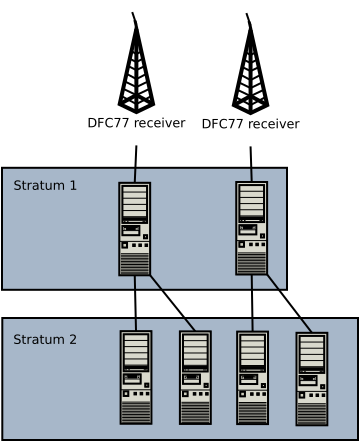
\includegraphics[width=0.33\textwidth]{Stratums}
\end{wrapfigure}

NTP is een hi\"erarchische structuur opgedeeld in stratums\index{Stratum}. Een \textquote{stratum 1} server is een server die direct gekoppeld is aan een referentieklok (atoomklok, DCF77 of GPS). De referentie klokken zijn stratum 0. Een server die zijn tijd haalt van een stratum 1 server heet een stratum 2 server. Een tijdserver die zijn tijd haalt van een stratum 2 server heet dan logischerwijs een stratum 3 server. Dit gaat zo door tot maximaal stratum 16.

Hoe hoger het stratum nummer hoe meer de tijd afwijkt van de tijd van de referentieklok. Middels berekeningen en onderlinge synchronisatie van servers in een bepaald stratum wordt deze onnauwkeurigheid zoveel mogelijk beperkt.

